%%%%%%%%%%%%%%%%%%%%%%%%%%%%%%%%%%%%%%%%%%%%%%%%%%%%%%%%%%%%%%%%%%%%%%%%%%%%%%%%
%2345678901234567890123456789012345678901234567890123456789012345678901234567890
%        1         2         3         4         5         6         7         8

\documentclass[letterpaper, 10 pt, conference]{ieeeconf}  % Comment this line out if you need a4paper

%\documentclass[a4paper, 10pt, conference]{ieeeconf}      % Use this line for a4 paper

%\IEEEoverridecommandlockouts                              % This command is only needed if
                                                          % you want to use the \thanks command

\overrideIEEEmargins                                      % Needed to meet printer requirements.

% See the \addtolength command later in the file to balance the column lengths
% on the last page of the document

% The following packages can be found on http:\\www.ctan.org

%\usepackage{epsfig} % for postscript graphics files
%\usepackage{mathptmx} % assumes new font selection scheme installed
%\usepackage{times} % assumes new font selection scheme installed
%\usepackage{amsmath} % assumes amsmath package installed
%\usepackage{amssymb}  % assumes amsmath package installed

\usepackage{graphicx}
\graphicspath{{images/}}

\title{\LARGE \bf Interprocess Communication for Robotics Applications
}

\author{Edward M. Roderick}

\begin{document}



\maketitle
\thispagestyle{empty}
\pagestyle{empty}


\begin{abstract}

Modern robotic systems are developed as a collection of independent processes. For these processes to function together, an interprocess communication system (IPC) must be implemented. Many prebuilt systems are available and this paper presents four popular options (Sockets, ZeroMQ, ACH, and ROS) as candiates for robotics. An analysis is presented for each based on communication latency and design metrics as applied to robotics. An example design is presented with analysis of the IPC selection process.

\end{abstract}





\section{INTRODUCTION}

As modern robotic systems grow in complexity, it becomes increasingly beneficial to implement a multi-process control system. This provides a modular system architecture. A modular architecture protects the overall system from individual components failing\cite{ACHLIBRARY}. Critical system processes can be allocated additional resources to ensure continued operation during a partial system failure. By predefining the inputs and outputs for each subsystem, multiple teams of designers can use differing languages, allowing for optimization of each task. Additionally, the overall system can be distributed across a variety of hardware (full computers, single board computers, micro-controllers)\cite{REALTIMEACH, EMBEDDEDROS, ACHHUBO}. 

Many IPC options are available to designers and each must be evaluated on a per system basis to determine the best candidate. This paper will focus on evaluating several mainstream options and how they apply to design metrics of robotic systems. As robots operate in real time, the latency and data integrity of each communication step is of critical importance\cite{IPCS}. For complex systems (humanoids, robots operating in proximity with humans, etc) with multiple processes running concurrently, communication delay can results in actuators responding to obsolete data\cite{ACHHUBO}. This paper serves to provide a guide to evaluating the capabilities of Sockets, Shared Memory, and ROS. 

\section{BACKGROUND}

\subsection{ACH (Shared Memory)}

POSIX IPC offers three types of messages: streams, datagrams and shared memory. For the real time robotics application, it is important to ensure that the IPC system is non head of line blocking as the most recent sensor data will take priority over previously acquired data. Streams suffers from head of line blocking and is thus not a desirable method for robotics. Datagrams utilize a data buffer that when full, loses any new data. This is particularly problematic as the robot would routinely lose important data. Shared memory is the fastest method of the POSIX suite and will provide the most current data by overwriting any old information stored. Unfortunately this method is susceptible to synchronization issues and further considerations must be taken in code which would reduce its reusability and complexity. Furthermore, for a realtime system, none of the POSIX IPC methods allow any methods of priority inheritance which is critical to allow high priority systems to access data first.

The ACH system allows the system to create multiple data channels to send data between processes. Each channel consists of two circular buffers: a data buffer and an index buffer. The two buffers are written in a channel specific POSIX shared memory file. By storing the data buffers in shared memory, the synchronization issue can be solved once for the entire channel via a mutex, allowing each reader process to poll the channel or wait for new data to be posted. This also prevents starvation and allows for priority inheritance between the real time processes.

A case study is presented \cite{REALTIMEACH} in which a balancing bipedal robot was developed with many different processes and ACH channels. The study details how the multiprocess approach allows for high priority processes (like balancing in this case) to stay alive in the event that other processes fail (ie computer vision). This approach also allowed processes to be distributed between smaller microcontrollers to drive servomotors to higher powered computers to process computer vision. SPIN simulations were run to benchmark the ACH system and it was shown that performance is identical to POSIX for single readers and receivers and the majority of the latency is a product of context switches. 



\subsection{Sockets: TCP and UDP}

placeholder for tcp and udp backgrounds

\subsection{ZeroMQ}

ZeroMQ (ZMQ) is a messaging system that extends on the foundations of sockets. It provides an additional abstraction layer over TCP by sending messages to a system topology instead of specific IP addresses. ØMQ prevents sending to specific IP addresses by design. The available messaging patterns is open ended, popular systems include publish/subscribe and request/reply. Only one messaging pattern is allowed for a topology and they cannot be interconnected. 

\begin{figure}[p]
    \centering
    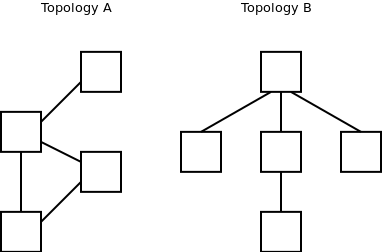
\includegraphics{zmqtopology}
    \caption{test}
    \label{test}
\end{figure}

This is essential to providing guarantees that data will arrive at its intended location. ØMQ separates its stack into end to end and hop by hop layers. Unlike TCP/IP, each ØMQ end to end protocol has its own hop by hop protocol\cite{ZMQTHEORY}. This allows each specific messaging pattern to have their own routing functionality. This allows bidirectional messages to be sent to specific nodes in the topology. Each intermediary node can determine if downstream sections of the network are unreachable and can signal the original client to resend now or wait until connectivity has been reestablished. 

With multicore processors being commonplace in today’s market and the growing availability of multicore processors in commercially available embedded systems there is a need for efficiently written multithreaded code. Current methods of dealing with the issues that arise from multithreading (synchronization, starvation, priority inversion) are difficult to learn and do not scale well as the number of available cores increases. By creating code with too many locks, threads can block one another and the system can perform inconsistently depending on what system the program is running on. Writing lock free code can become susceptible to processors reordering instructions and the code again performing inconsistently. These multithreading approaches are API based and incorrect usage can often result in multiple threads blocking each other and the program essentially running as a single threaded process. 
ZeroMQ provides a solution to these issues by abstracting the more difficult lock free multithreading code behind its native message passing techniques and achieves simple multithreading by sending messages between threads. Being based on BSD Sockets, the code implementation is simple and intuitive for existing programmers, as well as being available for a multitude of programming languages. ZeroMQ is infinitely scalable as the number of available cores increases without any rewriting of existing code.

\subsection{ROS}

With the growing availability of cheap ARM processor systems, versions of ROS are being developed to provide a lower cost design than the traditional full-fledged Linux pc. ROS subsystems can be distributed over multiple ARM systems, allowing for more design flexibility, lower power consumption, and improved scalability. ROS allows for higher level systems to be separated from real time subsystems and other system critical functions. This allows for high priority systems to be simplified to reduce risk of failure. ROS was designed to support higher level robot functions instead of the control of individual motors/sensors/etc. Much of the integration of subsystems is left to the design as ROS does not support fieldbuses. 

Three architecture styles exist for the designing to embed the ROS system: Embedded PC, Proprietary system with interface, or use of ROS messaging and APIs. The embedded PC would require all control hardware of subsystems to be fitted to the PC itself. This provides smooth integration with ROS, but fails to offer real hard time support. Entire existing robots can be managed from ROS by configuring a translation function between the proprietary system and the embedded system. This abstracts the lower level programming and allows for the existing systems to operate in real time. The third architecture is focused on the IPC system for ROS, which operates on remote procedure calls and publish/subscribe support. 

The ROS IPC system allows for custom messages to be used and provides flexibility in configuring the embedded systems. Rosserial, rosc, and Rosbridge are common methods of passing these messages. Rosserial provides a proxy over a C++ client that can be ported easily to any system that supports the language, not required an OS. Rosserial provides a ROS-like API to publish, subscribe, offer and consume RPC services. Potential issues arise with the proxy becoming a bottleneck. Rosc allows for direct connection to the Ethernet and handles native ROS connections and messages. However, for embedded systems, the TCP/IP overhead may prove too overwhelming for low powered systems. Rosbridge provides dynamic socket and websocket access to the full capabilities of ROS




\addtolength{\textheight}{-12cm}   % This command serves to balance the column lengths
                                  % on the last page of the document manually. It shortens
                                  % the textheight of the last page by a suitable amount.
                                  % This command does not take effect until the next page
                                  % so it should come on the page before the last. Make
                                  % sure that you do not shorten the textheight too much.


%%%%%%%%%%%%%%%%%%%%%%%%%%%%%%%%%%%%%%%%%%%%%%%%%%%%%%%%%%%%%%%%%%%%%%%%%%%%%%%%
\section*{APPENDIX}

Placeholder for appendicies

\section*{ACKNOWLEDGMENT}

placeholder for acknowledgements


%%%%%%%%%%%%%%%%%%%%%%%%%%%%%%%%%%%%%%%%%%%%%%%%%%%%%%%%%%%%%%%%%%%%%%%%%%%%%%%%
\nocite{*}
\bibliographystyle{IEEEtran}

\bibliography{IPC}

\end{document}
